\documentclass[10pt,a4paper]{article}
\usepackage[utf8]{inputenc}
\usepackage{amsmath}
\usepackage{amsfonts}
\usepackage{amssymb}
\usepackage{makeidx}
\usepackage{graphicx}
\usepackage{parskip}
\usepackage[left=2cm,right=2cm,top=2cm,bottom=2cm]{geometry}
\author{Miguel Ángel Xamie Diaz Fuentes/Jimenez Cortes Raúl}

\begin{document}
\begin{center}
\begin{LARGE}
\textbf{INGENIERÍA MECATRÓNICA}\\
\end{LARGE}
{\large Sistemas Electrónicos De Interfaz}\\
\begin{figure}[hbtp]
\centering

\includegraphics[scale=0.80]{UPZMG_Mecatr_nica.png}
\end{figure} 
\begin{center}
\begin{LARGE}
EV-2-1-Diseño Del Puente H Transistores.
\end{LARGE}
\end{center}

\begin{Large}
\textbf{Alumnos}
\\\textit{Miguel Ángel Xamie Diaz Fuentes\\Raul Jimenez Cortez}
\textbf{\\Maestro}
\\\textit{Morán Garabito Carlos Enrique}
\textbf{\\Fecha de Entrega}
\\\textit{01/11/2019}
\textbf{\\Grupo}
\\\textit{4-B}
\end{Large}

\end{center}

\footnote{Universidad Politécnica De La Zona Metropolitana De Guadalajara} 

\newpage

\section{Objetivo}
En esta practica se obtendrá como resultado lograr que a través de el primer circuito que se hizo con optocopladores y relevadores ya que de ahí se imparte el puente H haciéndolo funcionar así activándolo con los relays para cambiar el tipo de giro del motor en sentido horario del reloj y anti-horario.

\section{Materiales}

\begin{itemize}

\item Relays.
\item Resistencias.
\item Fuentes de Poder.
\item Multímetro.
\item Leds.
\item Cables Duponk.
\item Protoboards.
\item Optocopladores.
\item Push Button.
\item IRF840.
\item Motor 5v.
\item Transitores 2n2222.
\item Arduino.


\end{itemize}

\section{Marco Teórico}

Un Puente en H es un circuito electrónico que generalmente se usa para permitir a un motor eléctrico DC girar en ambos sentidos, avance y retroceso. Son ampliamente usados en robótica y como convertidores de potencia. Los puentes H están disponibles como circuitos integrados, pero también pueden construirse a partir de componentes discretos.
Estructura de un puente H (marcado en rojo).
Los 2 estados básicos del circuito.

\begin{figure}[hbtp]
\centering
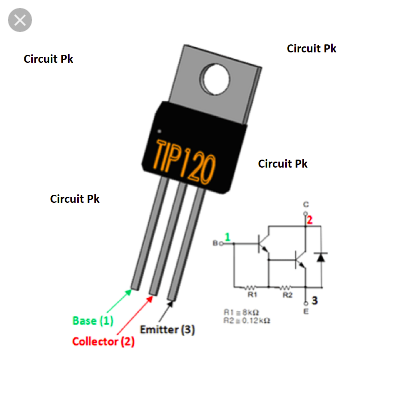
\includegraphics[scale=0.5]{1.png}
\caption{(S1-4 referidos a los diagramas) }
\end{figure}

El término "puente H" proviene de la típica representación gráfica del circuito. Un puente H se construye con 4 interruptores (mecánicos o mediante transistores). Cuando los interruptores S1 y S4 (ver primera figura) están cerrados (y S2 y S3 abiertos) se aplica una tensión positiva en el motor, haciéndolo girar en un sentido. Abriendo los interruptores S1 y S4 (y cerrando S2 y S3), el voltaje se invierte, permitiendo el giro en sentido inverso del motor.\\

\footnote{Universidad Politécnica De La Zona Metropolitana De Guadalajara} 

\newpage

Con la nomenclatura que estamos usando, los interruptores S1 y S2 nunca podrán estar cerrados al mismo tiempo, porque esto cortocircuitaría la fuente de tensión. Lo mismo sucede con S3 y S4. \\
\textbf{Aplicaciones}
Como hemos dicho el puente H se usa para invertir el giro de un motor, pero también puede usarse para frenarlo (de manera brusca), al hacer un corto entre las bornas del motor, o incluso puede usarse para permitir que el motor frene bajo su propia inercia, cuando desconectamos el motor de la fuente que lo alimenta. En el siguiente cuadro se resumen las diferentes acciones.\\



Tiene otras aplicaciones como generar un voltaje de salida AC a partir de controlar con dos PWM invertidos los Transistores s1, s2 y s3, s4. generando un voltaje alterno que se puede tomar diferentes frecuencias dependiendo del Duty-cycle que tomen las PWM. un ejemplo de esta configuración es el uso de un peltier para obtener una temperatura requerida en función de las PWM. \\

\textbf{Montaje:}
Lo más habitual en este tipo de circuitos es emplear interruptores de estado sólido (como Transistores), puesto que sus tiempos de vida y frecuencias de conmutación son mucho más altas. En convertidores de potencia es impensable usar interruptores mecánicos, dado su bajo número de conmutaciones de vida útil y las altas frecuencias que se suelen emplear.\\
Además los interruptores se acompañan de diodos (conectados a ellos en antiparalelo o sea, inversamente polarizados) como protección para los picos transitorios que generan las bobinas y otras cargas al desconectarse. puesto que el motor está compuesto por bobinados.

\footnote{Universidad Politécnica De La Zona Metropolitana De Guadalajara} 

\newpage

\section{Desarrollo}

\textbf{Etapa 1:}

Primero se realizo el circuito de acuerdo al diagrama dado por el profesor en clase un día antes de la practica para realizarla en físico. \\

Como seguimiento de esta practica se hizo el puente H en físico tanto como el diagrama del circuito ya que se fomenta así como se muestra en la siguiente imagen del diagrama ilustrando el motor con los IRF840 ya que también se pueden utilizar los transistores pero con estos se logro hacer y fomentarla.\\

\begin{figure}[hbtp]
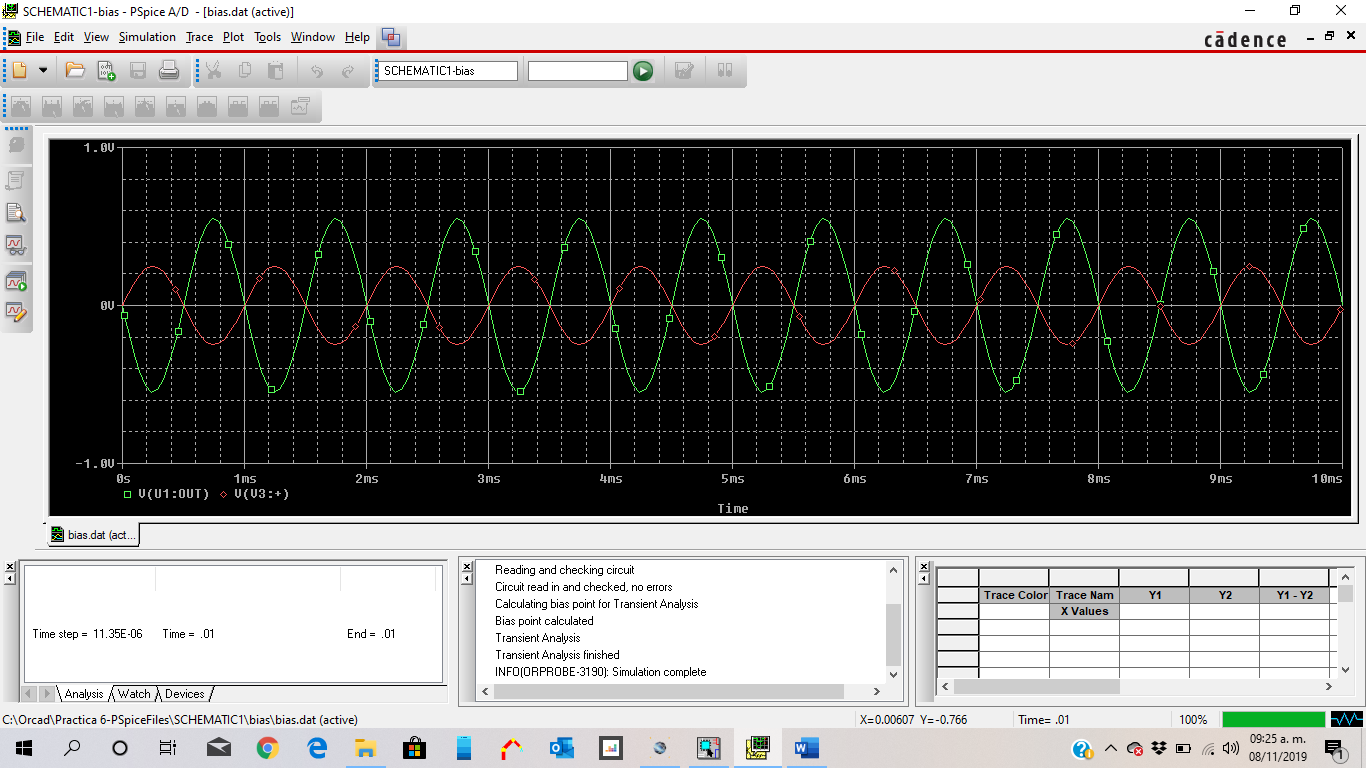
\includegraphics[scale=0.5]{2.png} 
\centering
\end{figure}
\begin{figure}[hbtp]
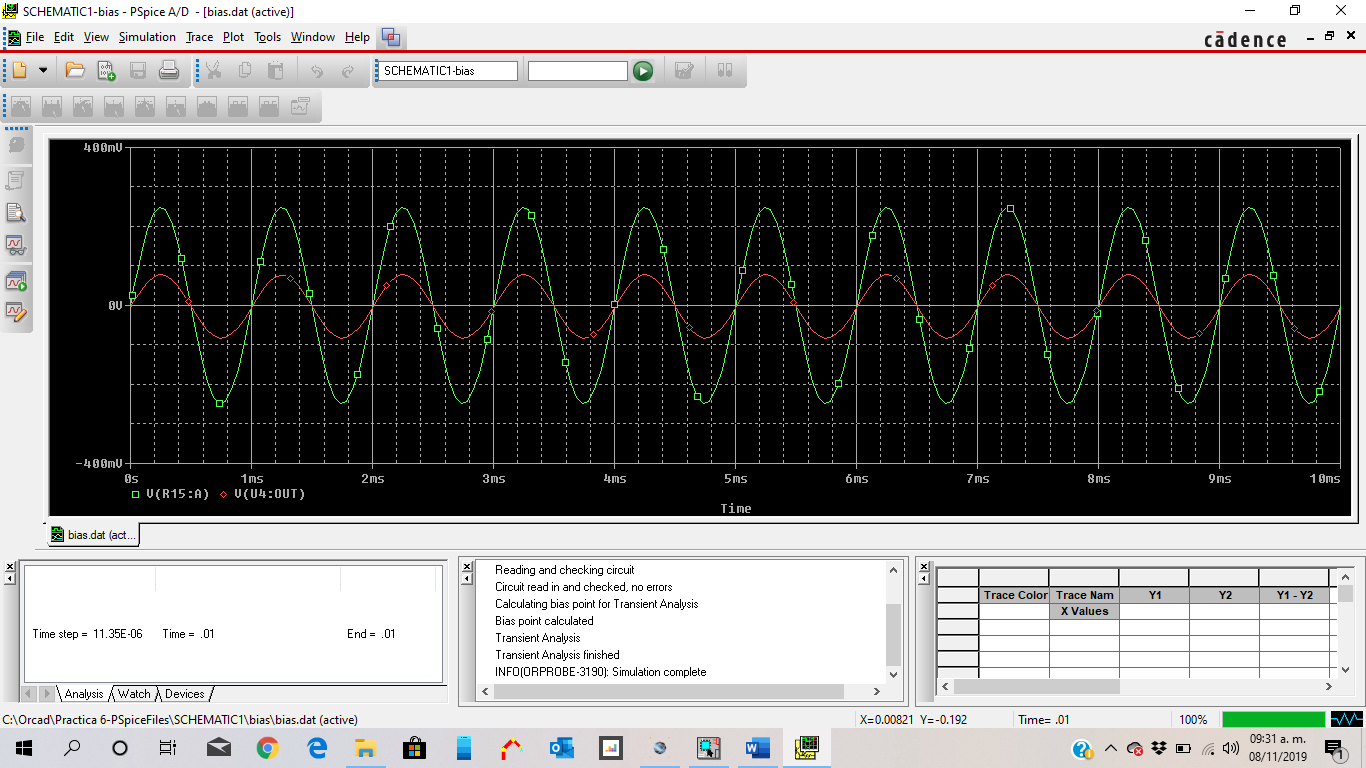
\includegraphics[scale=0.8]{8.png} 
\centering
\end{figure}
\textbf{Etapa 2:}

Después se ilustrara en la siguiente imagen donde se fomenta la primera parte del circuito donde sera activado por los relevadores junto con los optocopladores utilizando solo dos push button donde los relays activaran el puente H con el motor para hacerlo girar ya sea entre un sentido o otro.

\begin{figure}[hbtp]
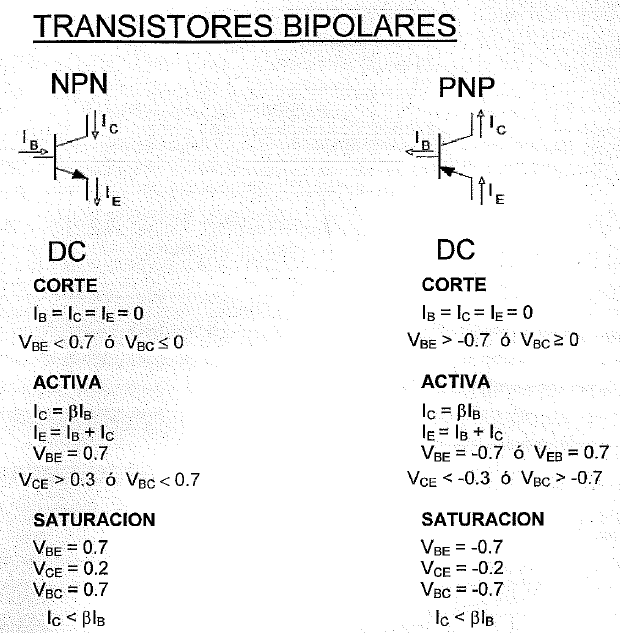
\includegraphics[scale=0.5]{3.png} 
\centering
\end{figure}

\footnote{Universidad Politécnica De La Zona Metropolitana De Guadalajara} 

\newpage

\textbf{Etapa 3:}

Como consiguiente de esta practica ya que se ilustra en las imágenes anteriores donde podemos ver como esta el circuito armado y una vez estando así, nos dios como resultado en que el motor lograra cambiar su sentido de giro tal cual le permite en su sentido horario y anti horario e así su entendimiento de lo que puede hacer un puente H ya en el area industrial solo que este es en pequeño, y ya que los push button vendrían siendo sus interruptores que van dirigidos u conectado con los relevadores y dar su frenado con tan solo cambiar u presionar el otro boto para su distinto giro.

A continuación se muestran algunas imágenes del circuito en físico y la parte de control con los relevadores.

\begin{figure}[hbtp]
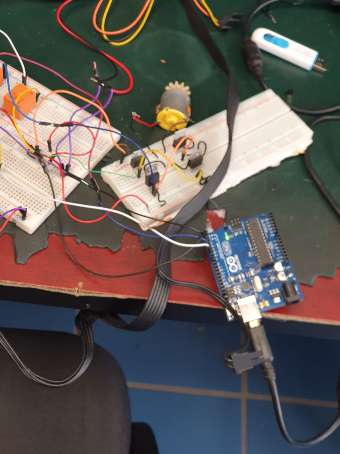
\includegraphics[scale=0.5]{4.png} 
\centering
\end{figure}

\begin{figure}[hbtp]
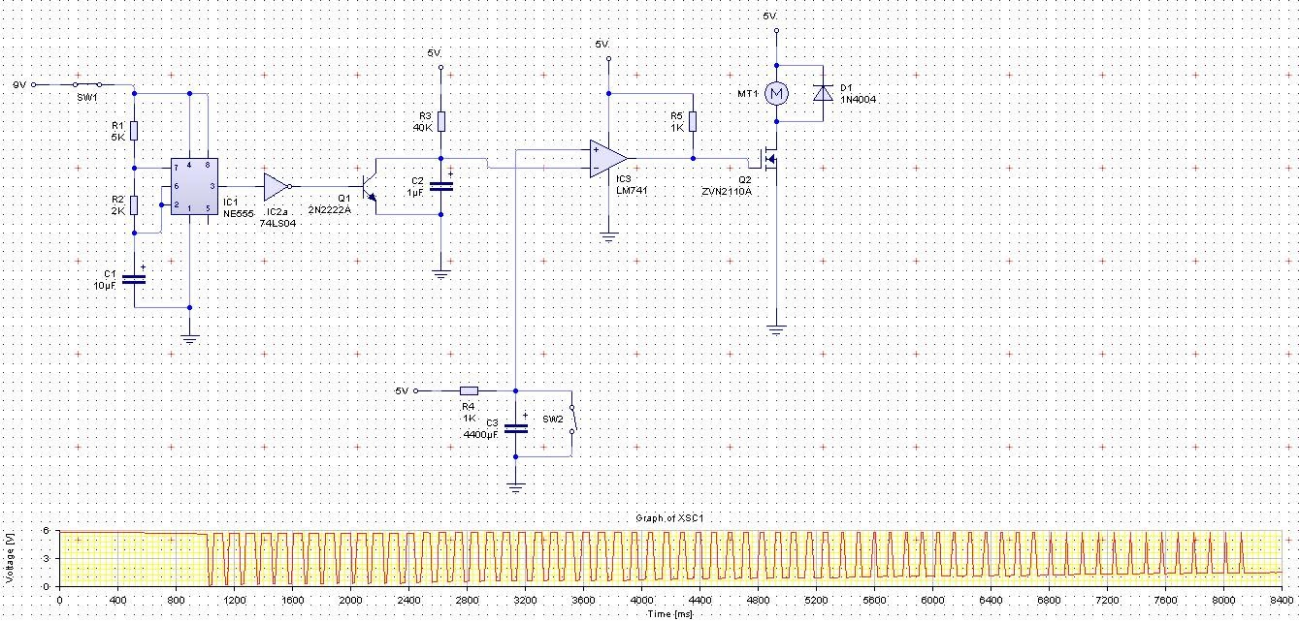
\includegraphics[scale=0.5]{5.png} 
\centering
\end{figure}

\footnote{Universidad Politécnica De La Zona Metropolitana De Guadalajara}
\newpage

\begin{figure}[hbtp]
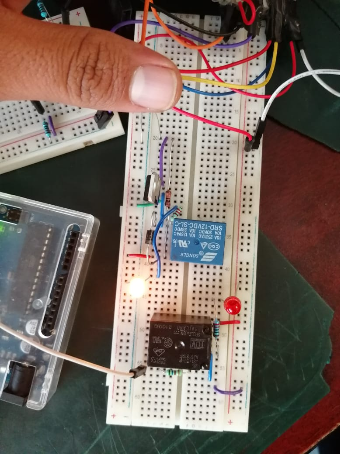
\includegraphics[scale=0.4]{6.png} 
\centering
\end{figure}


\section{Cálculos}

Para el uso de las resistencias correctas se realizaron cálculos de acuerdo al modelo del optoacomplador y una que esta en función de salida hacia el arduino y la recibe el transistor (2N2222).\\
Datos:\\

Voltajes de entrada: 12v, 5v.\\

Datos del optoacoplador:\\

If = 10mA ------
Vf = 1.12v\\

{\Large $ R_{Led} = {\Large \frac{(12v - 1.15v)}{10mA}}$} \\


\footnote{Universidad Politécnica De La Zona Metropolitana De Guadalajara}
\newpage

Aquí se toman los parámetros del optoacoplador (425).\\

{\Large $R_{Led} = 1.085\Omega$}\\

{\Large $R_{Transistor} = \frac{(5v - 0.6v)*250}{12mA}$}\\

Aquí se toman los parámetros del relevador y de la medida del transistor con el multimetro.\\

{\Large $R_{Transistor} = 1.528K\Omega$}\\

Por ultimo también determinamos la potencia.\\

$ W = I^2 R $\\ 

$ W = (10mA)(1.100\Omega)$\\

$ W = 0.11w $\\

\section{Conclusiones}
En esta practica se pudo entender el funcionamiento de un puente h ya que se usa para permitir a un moto girar en ambos sentidos de un avance o retroceso, ya que estos son ampliamente usados en distintos lugares ya sea como en la parte industrial porque son unos convertidores de potencia, el cual también en esta practica tuvimos algunas fallas pero era por cuestiones de que no giraba el motor, el cual era por la conexión incorrecta que teníamos la cual fue solucionada desarmando todo el circuito y probando cada mosfet activándolo y desactivándolo para entender correctamente como funcionan a su vez que se probaba el motor cada parte hasta que realizara la función de retroceso y avance como se lo pide la practica lo cual pudimos solucionar y se cumplió del objetivo.

\bibliography{Referencia}
\begin{thebibliography}{X}
\bibitem{Baz} Técnicas electrónicas digitales. A. Hermosa Donate. 1997
TECNOLOGÍA ELECTRÓNICA. L. Gomez de Tejeda.
ELECTRÓNICA ANALÓGICA. L. Cuesta, A. Gil Padilla, F. Remiro.
Técnología Electrónica. Tomás Pollán Santamaría.
H BRIDGE MOSFET Teoría de operación. E.U.C.A.M.
DUAL FULL-BRIDGE DRIVER L298 H BRIDGE ST. 
\end{thebibliography}

\bibliographystyle{plain}
\footnote{Universidad Politécnica De La Zona Metropolitana De Guadalajara}
\end{document}